\documentclass[a4paper]{../birkjour}

\usepackage{../fouche-copy}
\makeatletter
\def\@settitle{\begin{center}%
  \baselineskip14\p@\relax
  \bfseries
  \uppercasenonmath\@title
  \@title
  \ifx\@subtitle\@empty\else
     \\[1ex]\uppercasenonmath\@subtitle
     \footnotesize\mdseries\@subtitle
  \fi
  \end{center}%
}
\def\subtitle#1{\gdef\@subtitle{#1}}
\def\@subtitle{}
\makeatother

\newcommand{\var}[3][]{
  \left[\begin{smallmatrix} #2 \\
  #1\downarrow \\ #3
  \end{smallmatrix}\right]}
\newcommand{\cvar}[3]{
  \begin{xsmallmatrix}{0em}
  & #1 \\ #2 & \downarrow \\ & #3
  \end{xsmallmatrix}}

\def\la{\langle}
\def\ra{\rangle}
\def\lr#1#2{\la #1,#2\ra}
\def\tr{\textsf{t}}
\newcommand{\true}{\texttt{t}}
\def\id{\text{id}}
\author{Dario Dentamaro}
\address{Dario \textsc{Dentamaro}: }
\email{dio@cane.it}
\author{Fosco Loregian}
\address{%
  Fosco \textsc{Loregian}: %
  Tallinn University of Technology, %
  Institute of Cybernetics, Akadeemia tee 15/2,%
  12618 Tallinn, Estonia}
\email{fosco.loregian@taltech.ee}
\email{fosco.loregian@gmail.com}
\title{Categorical ontology I}
\subtitle{Existence}
\usepackage{proof}

\usepackage{minted}
\def\mil#1{\mintinline{haskell}{#1}}
\newcommand{\po}[1][dr]{\save*!/#1+1.5pc/#1:(1,-1)@^{|-}\restore}
\newcommand{\pb}[1][dr]{\save*!/#1-1.5pc/#1:(-1,1)@^{|-}\restore}


\setlength{\epigraphwidth}{.6\textwidth}
\setcounter{tocdepth}{1}

\usepackage{fontawesome}

\def\ang#1{\langle #1 \rangle}
\def\lsem{\textcolor{gray!60}{[}}
\def\rsem{\textcolor{gray!60}{]}}
\def\trn#1{\lsem #1\rsem}

\def\f#1{\textcolor{red}{#1}}
\let\phi\varphi
\newcounter{quad_i}
\newcommand{\qd}[1][]{\ifthenelse{\equal{#1}{}}{\quad}{\setcounter{quad_i}{0}\whiledo{\value{quad_i}<#1}{\quad\stepcounter{quad_i}}}}
\newcommand{\funsp}[2]{(#1 \Rightarrow #2)}

\newcommand{\fo}[1]{{\color{red} #1}}

\title{Categorical Ontology: Functorial \emph{Erkennen}}
%== authors' info
% \author{Blinded authors}
%
%
%
\author{Dario \textsc{Dentamaro}}
\address{Università degli Studi di Firenze,\newline Dipartimento di Matematica e Informatica
        }
\email{dario.dentamaro@stud.unifi.it}
% \email{dariodentamaro26@gmail.com}
%
\author{Fosco \textsc{Loregian}}
\address{ Tallinn University of Technology,\newline %
          Institute of Cybernetics, Akadeemia tee 15/2, \newline %
          12618 Tallinn, Estonia }
\email{fosco.loregian@taltech.ee}
% \email{fosco.loregian@gmail.com}


\usepackage{booktabs}

\newcommand{\bk}[1]{\langle #1\rangle}
\newcommand{\numberset}{\mathbb}
\newcommand{\N}{\numberset{N}}
\begin{document}

\begin{abstract}
	The present paper approaches ontology and meta\hyp{}ontology through Mathematics, and more precisely through the theory of \emph{elementary toposes}; for us, an \emph{ontology} is a mathematical object: it is a category $\clE$, the universe of discourse in which our Mathematics (intended at large, as a theory of knowledge) can be deployed. The well-studied \emph{internal language} of such categories is expressive enough to talk about existence, sometimes in a nuanced way that is akin to the way in which different philosophers talked; technically speaking, the presence of an object $\Omega_\clE$ parametrizing the truth values of the internal propositional calculus prescribes the `modes of existence' for the objects of a fixed ontology/category.

	This approach resembles, but is more general than, the one leading to \emph{fuzzy logics}, as most choices of $\clE$ and thus of $\Omega_\clE$ yield nonclassical, many-valued logics.

	As both a test-bench for our theory, and a literary \emph{divertissement}, we propose a possible category-theoretic solution of the famous Tl\"on's ``nine copper coins'' paradox, and of other seemingly paradoxical construction in Jorge Luis Borges' literary work.

	We conclude with some vistas on the most promising applications of our future work.
\end{abstract}
\maketitle

{\footnotesize\tableofcontents}
\newpage

\fo{Todo list
  \begin{itemize}
    \item l'introduzione;
    \item unire un po' prima metà e seconda metà
    \item limare l'intro
    \item rileggere tutto
  \end{itemize}
}
\epigraph{[\dots\unkern] Le rôle essentiel c'est cette transition qu'il y a entre ce quelque chose qui est écrit, qui parait incompréhensible, et les images mentales qui l'on crée.}{A. Connes}
\section{Semantic conception of theories}\label{sec_1_intro}
The present work approaches a well-established problem in epistemology: what is the way in which we build representations of the world from perception? What is, if any, the relation between the two `worlds', one depicted in our minds, and one on our fingertips? Sometimes, such a representation results in a faithful image of the perceived world (we call it `science'); sometimes it doesn't (we call it `superstition'). 

We propose a sense in which science and superstition can be told apart using a mathematical theory, or even a mathematical object.
\subsection{A convincing notion of theory: two dictionaries}
Along the XXth century there have been many attempts towards a formal definition of a scientific theory. 

Examples are the \emph{Wiener Kreis}' verificationist paradigm, and Neurath's theory of `protocollar statements', that gave an initial input towards the elaboration of a semantic framework for scientific theories, and spurred the search for a pan-linguistic vision of philosophy of science \cite{Weinb}.

The formal account in which --among others-- Carnap \cite{carnapfound} provided his notion of `theory' is known in the literature as \emph{syntactical conception of theories} or `received view' \cite{krause-foundation,krause2011axiomatization,giunti2016}. Albeit the term `semantic' is due to later developments, the field of epistemology that logical neopositivism started can legitimately be labeled a `semantics of theories', because some of its features, if not the underlying ideology, are the same throughout the work of Carnap \cite{carnap56,carnapfound},  Beth \cite{?}, and Suppe \cite{suppe89}.

Thus, a `Wiener Kreis' theory' is understood as a structure $(F_\clL, \clK)$ where $F_\clL$ is a formal language, and $\clK$ the totality of all its interpretations, or \emph{models}. 

The idea to separate further $F_\clL$ into two `vocabularies' $(\clT,\clO)$ (intended, in modern terms, as two syntactic categories carved from two first order theories) first appears in Carnap \cite{}; these are respectively the \emph{pure} or $\clT$\emph{heoretical} terms, and the \emph{applied} or $\clO$\emph{bservational} terms \cite{refs_on_erkennen}. 

It is a commonly accepted belief --albeit rarely formalised-- that scientific theories arise from some kind of tension between the theoretical and the observational world. Our aim here is to try and `resolve the tension', acknowledging $\clT,\clO$ and their mutual relations as concrete mathematical object, rooted in category theory \cite{McL,pedicchiofoundations,riehlcontext,leinster2014basic}.

As elementary as it may seem, this idea seems fruitful to us: building on Carnap, 
\begin{remark*}
	A reasonable notion of `scientific theory' is a triple $\bk{(\clT,\clO), \clK}$ whose first two elements form the `underlying logic' $F_\clL=(\clT,\clO)$ and where $\clK$ is a (possibly large) category of models or `interpretations'. 
\end{remark*}
This is in fact a familiar old idea for mathematicians, as the habit of identifying a sort of mathematical structure in a way that is independent from the cohort of its syntactic presentations, permeates classical universal algebra since the early work of Lawvere \cite{lawvere1963functorial,lawvere1996unity} (see also \cite{abramskyno,Borceux1994,makkai1989accessible} for applications to logic and other disciplines).

% Tangentially, a similar syntax-semantics approach appears in \cite{biologia} to axiomatise a notion of `evolutionary theory'; the connection between the intrinsic logic of living systems is not peregrine: in passing, we mention that the pioneering work of R. Rosen --a survey of which is given in \cite{letelier2006organizational}-- extensively uses category theory.
% \begin{definition}[Wiener Circle theory] \cite{krause-foundation}
% 	A theory $T$ consists of:
% 	\begin{itemize}
% 		\item A formal language $\clF_\clL$ formed by a non-logical vocabulary $\overline{\clV}$, which is further divided into two sub-vocabularies: $\clT$ for theoretical terms and $\clO$ for observational terms.\footnote{There are no restrictions on the choice of language here:
% 			      \begin{quotation}
% 				      one already commits the theory with being characterized not only by its postulates and correspondence rules but also with a specific vocabulary and language. [...] Given that a theory is identified with its linguistic formulation (in axiomatic terms), it would result in impossible formulations of the same theory in alternative vocabularies. \hspace{\fill}\cite{krause-foundation}
% 			      \end{quotation}}
% 		\item A logical vocabulary, namely a set of logical axioms endowed with derivation rules and a notion of consequence relation, called $\clV$. So $\clF_\clL= (\clT,\clO) \cup \overline{\clV}$.
% 		\item A set of sentences in $\clT$ called \emph{theoretical postulates}.
% 		\item An informal semantics for observational terms whose relating terms of $\clO$ with observable objects and events \footnote{Questo è fortemente dipendente dalla meaning theory neopositivistica \cite{} ed è un passaggio problematico per motivi chiariti più avanti}.
% 		\item A set of sentences called \emph{correspondance rules} relating theoretical terms with observational terms.
% 	\end{itemize}
% \end{definition}
In the Carnapian --and in general the neopositivistic-- account a theory can be expressed as a sentence formed by terms $\tau_1, \dots, \tau_k$ taken from both the dictionaries of $F_\clL$.

In the Wiener Kreis paradigm, the formal specification of $\clO$ is left unclear; Carnap \cite{carnapfound} posits the existence of \emph{correspondence rules} between $\clO$ and $\clT$, associating to each term $o$ of $\clO$, or O-term, its companion in $\clT$, or the T-term $\tau$ derived from $o$. In general, Carnap holds that $\clO \subset \clT$, but at the same time he blurs the features of this identification of observational terms as `types of T-terms'.

We can maintain a similar idea, just phrased in a slightly more precise way: we posit the existence of a function $\varphi$ that translates O-terms into T-terms. So, a Wiener definition of a theory is a suitable set of pairs $\{\bk{\tau,\varphi(\tau)} \mid \tau\in\clT\}\subseteq \clT\times\clO$, where $\varphi: \clT \to \clO$ is called a \emph{translation function}. In this way it is trivially true that all the terms of a theory are in the first dictionary. 
\begin{remark*}
	A reasonable notion of scientific theory must take into account `meaningful relations' between the observable world $\clO$ and the theoretical world $\clT$; the Carnapian request that there is a functional correspondence between the two is, however, too restrictive when $\clT,\clO$ are thought as categories.
\end{remark*}
In fact, the set of pairs of a Carnap translation function $\varphi$ is precisely the \emph{graph} of $\varphi$, and not by chance: cf. our \autoref{da_collage}.\footnote{In passing, it is worth to notice that Carnap's intuition fits even more nicely in our functorial framework: assume $\clT, \clO$ exhibit some kind of structure, and that $i : \clO\subseteq\clT$ \emph{as substructures} (e.g., assume that they are some sort of ordered sets, and that the order on $\clO$ is induced by the inclusion); then, a \emph{left} (resp., \emph{right}) \emph{translation function} $\varphi_L$ (resp., $\varphi_R$), is a left (resp., right) adjoint for the inclusion $i : \clO\hookrightarrow \clT$. We will not expand further on this idea, but see \autoref{carnap_translation_functors}.}

Now, the neopositivistic current of epistemologists was the first to observe that one can build an observational version of a theory $T$ following a procedure first outlined by Ramsey \cite{?} and colloquially called \emph{Ramseyfication} of a theory; the nature of this operation seems quite elusive to those approaching it: colloquially, it can be thought as the process of replacement of each observational term of a theory with a `corresponding' theoretical term. The nature of this replacement, the syntactic domain of terms, and the sense in which the process makes a theory $F_\clL$ and its `Ramseyfied' analogue $F_\clL^\text{Ra}$ equivalent are however quite elusive.

In the language of category theory --and especially through our profunctorial approach-- instead things become clearer: under mild assumptions on a diagram 
\[ \vcenter{\xymatrix{
	& \clW \ar[dl]_{N_\phi} \ar[dr]^{N_\psi} & \\
	[\clT^\op,\Set] \ar[rr]_{N_{\hat R}} && [\clO^\op,\Set]
	}} \notag\]
of categories and profunctors, if a `deduction' entails a certain interaction or a certain behaviour for the theoretical category over the observational one, then there exists a particularly well behaved natural transformation 
\[ \varpi : N_{\hat R} \To \bk{\phi/\psi}\notag \]
filling the triangle above; in non\hyp{}mathematical terms, this means that the entailment of a theoretical prediction into an observed system (i.e. a term $\tau$ of type $\fkR(T,O)$) yields an entailment $\varphi(T) \to \psi(O)$ \emph{in the world}. The details of this construction, that we consider the heart of the paper, are contained in \autoref{inducing_herme}, \autoref{funcell_herme}, and heavily rely on the terminology introduced in Sections \ref{sec_2_profu} and \ref{sec_3_nervi}.

The next subsection offers a birds-eye view of the structure of the paper.
% \color{red}

% Tutta la parte che ho commentato mi sembra goffa e confusa; io svilupperei la discussione come ho fatto sopra, e proseguirei in modo simile: svelando man mano di cosa deve esser fatta la teoria che andiamo a costruire; primo, deve essere fatta di una coppia di categorie T, O con certe proprietà; secondo, deve esserci una relazione tra loro, perché una funzione è troppo restrittiva; questo motiva già quasi tutto. Da questo, osserviamo che il tentativo di Ramsey è essenzialmente un tentativo fallito, ma tentiamo di salvare il salvabile. Nella nostra formulazione, infatti, l'operazione acquista un senso in termini di una prop univ; questo è il cuore del lavoro, e si presta ad alcune osservazioni: 

% 1. la distinzione tra teorico e osservazionale è fittizia, e questo si riflette nel modello profuntoriale

% 2. abbiamo un discrimine, se non universale, perlomeno abbastanza concreto per distinguere l'astrologia dalla meccanica quantistica; e per contro, la cosmogonia di Tolkien è perfettamente `scientifica'.
% \color{violet}
% Now, the neopositivistic current of epistemologists was the first to observe that one can build an observational version of a theory $T$ following a procedure first outlined by Ramsey \cite{?} and colloquially called \emph{Ramseyfication} of a theory; among many different attempts at an axiomatization of this formal procedure, we feel the following is the most suited for our analysis, and the easiest to justify:%approaching the relevant literature on the subject, such a procedure  La Ramsey-sentence of a theory, non potendo nessun termine $\tau_k \in \clF_\clL$ uscire da $\clT$, sia un ri-tradurre nel linguaggio di $\clO$ il contenuto della teoria, sostituendo i termini teorici "puri" con delle variabili (dimenticando di specificare un dominio di oggetti da cui prenderle).
% \begin{definition} [Ramsey sentence]
% 	Let $F = (\clT,\clO)$ be a theory, and $\varphi: \clT \to \clO$ a translation function; the \emph{Ramseyfication $F^\text{Ra}$ at a term $\xi\in\clT$} of $F$ is obtained as
% 	\[
% 		F^\text{Ra} = \{\bk{[\tau/\xi], \varphi([\tau/\xi])} \mid \tau\in\clT\}
% 	\]
% \end{definition}
% One says that $F^\text{Ra}$ represents the \emph{observative content} of $F$. 

% This can be seen as a way to circumvent the fact that no theoretical term $\tau$ can really `exit' the theoretical category $\clT$; however

% \medskip
% We find no epistemological motivation to follow such an approach (were it only because it is cumbersome, and it raises more questions than it is able to solve);  Non ci pare, al netto degli obiettivi riduzionistici del Wiener Kreis \cite{}, che ci siano motivi epistemologicamente validi per eseguire un tale procedimento, che del resto non ha avuto molto seguito nella letteratura successiva, ma la distinzione carnapiana è ripresa nel nostro framework, per trarre alcune conclusioni on relations between theoretical and observational core \autoref{sec:orge11c3c4} e su come allargare la nozione stessa di teoria \autoref{}.

% I termini di $\clO$ si riferiscono a fenomeni ma sono appunto 'termini': anche nei futuri sviluppi semantici il trattamento formale impedisce di uscire davvero dalla sintassi. Parafrasando Duhem si potrebbe dire che già agli albori della semantics of theory "tutta l'osservazione [in fisica] è carica di teoria" dove per teoria si intende la categoria sintattica $\clT$.

% Le ambiguità carnapiane sul dominio di oggetti sui quali verterebbe la definizione viennese noi, coerenti col testo, le risolviamo indicando come dominio $\clT$. Cosa sia il mondo puro delle osservazioni al quale farebbe riferimento la Ramsey-version della teoria non è chiaro, se non un altro sotto-dizionario teorico, per l'appunto. Non a caso il neopositivismo da un iniziale fisicalismo approda ad un'ottica convenzionalista \cite{?}, in seguito ai falliti tentativi di formalizzazione di un contesto osservazionale extra-teorico.

% Seguendo \cite{psillos} si può dare una lettura strutturalista a questi attempts. Si può dire che una teoria $T$ is logically equivalent to the conjunction
% \[T^\text{Ra} \land (T^\text{Ra} \rightarrow T)
% \] where the second member is the \emph{meaning postulate}:
% \begin{quotation}
% 	Carnap notes that this conditional has no factual content and takes it to be a meaning postulates \cite{psillos}
% \end{quotation}

% This is a kind of 'if-then' realism: the subject of study of scientific knowledge is not the world, but instead the conditions that, given certain assumptions, happen to be true in the structural world that the theories describe.

% The meaning postulate is nothing but the Wiener Kreis' version of the famous \emph{demarcation problem} between science and metaphysics: the attempt to elaborate a distinguishability criterion between a proposition belonging to empirical sciences, and a metaphysical (or, more broadly, a non-scientifical) one. Such criteria have always been either too strict (taking sensorial experience as ultimate judge of a scientific statement), or too large (from \cite{schwarz2009twisted}: \emph{Physics is a part of Mathematics devoted to the calculation of integrals of the form $\int g(x) e^{f(x)}dx$}): our approach addresses this problem.

% Tolti i due estremi, gli enunciati protocollari da un lato \cite{?}, i discorsi di Heidegger dall'altro \cite{?}, esistono tutti i casi intermedi per i quali a meaning criterion (o una operazione come la drastica traduzione dei costrutti teorici in "referti osservativi puri" tramite ramseyfication) impedisce concretamente di individuare la demarcazione.
% %Classical objections range from Popper \cite{?} to more recent sociology of science.

% Negli anni, oltre a tramontare le aspirazioni fisicaliste della cosiddetta received view, si sono dissolti anche gli approcci generali al problema del trattamento formale delle teorie scientifiche, e si sono moltiplicati gli studi su linguaggi specifici dell'impresa scientifica \cite{}.

% Proveremo che a profunctorial approach è un modo per riconsiderare nozioni più larghe e 'universali', costeggiando anche il demarcation problem. In più chiarendo come si induce una interpretazione sulla categoria 'mondo' e quale ruolo svolgono le versioni funtoriali degli strumenti classici di questo campo, fin qui criticati \autoref{inducing_herme}.
\color{black}
\subsection{Our contribution}
The first remarks that we made in the introductory subsection motivate at least our tentative definition for a `pre-scientific' theory: it is some sort of correspondence of categories $R : \clT \pto \clO$, between an observational and a theoretical category.

Another important point throughout the above discussion however is that from a neo-positivistic stance the distinction between theoretical and empirical is purely formal.

This is not due to the hypothetical nature of the former (empirical laws can be hypothetical), but to the fact that the two kinds of law contain different types of terms, as first observed in \cite{carnap56}. This purports a purely linguistic approach to epistemological issues, that we want to take at the extreme.

In fact, our work pushes in this direction even more: the profunctorial formulation of scientific theories deletes even more forcefully any intrinsic distinction that might be between the observational and the theoretical\fshyp{}linguistic structure of a theory.

In profunctorial terms, thanks to \autoref{da_collage} and standard category\hyp{}theoretic arguments, there is a direct counterpart \emph{in the mathematical model} for the vanishing of the distinction between observational and theoretical.

First of all, the bicategory defined in \autoref{def_profu}, taking from \cite{benabou2000distributors}, is self-dual; this means that every profunctor $\fkR : \clT \pto \clO$ admits a `mirror image' $\fkR^\op : \clO \pto \clT$;\footnote{This is reminiscent of the fact that, as observed in \autoref{sec:org7dd09e1}, a relation has not a privileged domain of definition; clearly, the category $\mathsf{Cat}$ has a nontrivial involution given by $\op$ing a category, and this renders the auto-duality slightly more visible in the case of categorified relations (i.e., profunctors).} second, and certainly more decisive a comment towards our thesis, as outlined in \autoref{resoudre_la_tension} a generic profunctor $\fkR : \clT \pto\clO$ yields the `collage' of the observational and theoretical categories $\clT,\clO$ `glued along' $\fkR$; in simple terms, the collage of $\clT,\clO$ along $\fkR$ is a new category $\clT\uplus_p\clO$, fitting in a span
\[ \vcenter{\xymatrix{
			& \clT\uplus_p \clO \ar[dr]\ar[dl]& \\
			\clT  && \clO
		}} \] having suitable fibrational properties (cf. \autoref{def:dfib} and in particular \autoref{collage_explaned}) allowing to recover the theoretical and observational terms as `lying over' $(T,O)\in\clT\times\clO$.

From this perspective, it seems obvious why we require the pair $(\clT,\clO)$ to admit a profunctor in either direction; profunctors categorify the notion of `meaningful relation' between structured high-level systems, i.e. two syntactic categories $\clT,\clO$ `modeling' the environment to which we have access.

Proposing the fundamental features of a `general theory of scientific theories' stated in terms of profunctors is the main contribution of the present work.

\medskip
We conclude this introductory section with a paragraph discussing about the `nature'' of the categories $\clT,\clO$, while surveying on the main arguments of the paper.
As we already observed in a previous work \cite{catont1}, the problem of locating the syntactic objects embodying a linguistic theory can be easily solved from an esperientialist stance: the world undeniably exists, and it is a sufficiently complex structure to contain the concrete building blocks of a formal system. We derive the primitive symbols of language from a portion of the world, complex enough to offer expressive power.

This problem, and its proposed solution, reflect unavoidably on the way in which the categories $\clT,\clO$ are built. In our model the world is a (possibly large) category $\clW$, unfathomable and given since the beginning of time, to which we can only access through \emph{probe maps} (functors) $\phi : \clL \to \clW$ (cf. \autoref{canvas_scienza}) representing small `accessible' categories construed from parts of $\clW$ that we can experience.

The request that $\clW$ is `sufficiently expressive' now translates into the request that as a category $\clW$ contains enough traces of functors like $\phi$; this (cf. \autoref{mondo_yalda}) translates formally in the request that any such $\phi$ admits a \emph{colimit} (cf. \cite[Ch. 2]{Bor1}) in $\clW$.

When things are put in this perspective, a few remarks are in order:
\begin{itemize}
	\item This perspective allows to close the circle over the problem of representation of a world $\clW$ in terms of a portion $\clT$ to which we have hermeneutical access, and from which we have carved a language.

	      In fact, such a representation happens through `canvas functors' $\phi : \clL \to \clW$ that, thanks to the cocompleteness property of $\clW$, extend uniquely to representation functors $[\clL^\op,\Set] \leftrightarrows \clW$.
	\item On the other hand, `the world' as a whole is unknowable: instead of $\clW$, we can access to an observational fragment $\clO$, from which we recover, exploiting the cocompleteness of $[\clO^\op,\Set]$, a further representation $[\clL^\op,\Set] \leftrightarrows [\clO^\op,\Set]$. In general, this is all that can be said; such a picture is already capable of determining, by elementary means, an equivalence of categories (i.e., an equivalence of models) between the observational and the theoretical \emph{nuclei} of $[\clT^\op,\Set] \leftrightarrows [\clO^\op,\Set]$: we discuss the matter in \autoref{nuclei}, and \autoref{resoudre_la_tension}.
	\item Additional assumptions on the canvas $\phi : \clL\to \clW$, however, can refine our analysis: we can infer that the totality of models $[\clL^\op,\Set]$ \emph{contains a copy} of the world $\clW$. In this precise sense, assuming what is outlined in the definition of \science in \autoref{canvas_scienza}, language prevails: the unfathomable world is a full subcategory of the class of all modes in which the language of $\clT$ can be interpreted.
	\item Under very mild assumptions on the arrangement of functors
	      \[\notag\vcenter{\xymatrix{
		      & \clW \ar[dr]^{N_\psi}\ar[dl]_{N_\phi} & \\
		      [\clT^\op,\Set] \ar[rr]_{N_{\hat R}} && [\clO^\op,\Set]
		      }}\]
	      (cf. \autoref{nervereal}) where $\phi,\psi$ are two canvases, respectively on the theoretical and observational side, we can find a natural 2-cell filling the triangle; this amounts to a `concretisation' of the canvases (see \autoref{funcell_herme} and \autoref{herme_explained}) into an implication between (a trace that) the theoretical terms (left in the world via $\phi$) and the observational terms (to which we have experimental access) in $\clW$. This last sentence is `the Ramsey sentence' that the canvases carve into the world, expressed in the internal language of $\clW$.
\end{itemize}
% As bold a statement as it might seem, this has fruitful consequences: see for example \autoref{remark_yuggoth_1}, \autoref{remark_yuggoth_2}.
\subsubsection*{Structure of the paper}
Section \ref{sec_2_profu} and \ref{sec_3_nervi} outline the mathematical background we need throughout the work; section \ref{sec_4_theories} introduces our main notions: a canvas, a world, a theory, a science. Sections \ref{sec_5_tension} and \ref{sec_6_universal} will conclude the discussion.%, towards an evidence that the two dictionaries, theoretical and observable, live in a very tight relation; a broadly intended notion of \emph{theory} asks for a precise understanding of the category of adjunctions between the theoretical and observational side.
\section{Profunctors and the Gro\-then\-dieck construction}\label{sec_2_profu}
\label{sec:org7dd09e1}
We start from a simple observation.
There are two possible ways to define a relation $R$ between two sets $A,B$:
\begin{enumtag}{r}
	\item \label{r_1} a relation $R$ is a subset of the cartesian product $A\times B$;
	\item \label{r_2} a relation $R$ is a function $A\times B \to \{0,1\}$.
\end{enumtag}
This notion of `relation between $A$ and $B$' is inherently symmetric, in the sense that such $R$ can be regarded both as a kind of map $A \rightsquigarrow B$ or $B\rightsquigarrow A$.

Furthermore, every relation $R$ between sets $A,B$ gives rise to a \emph{Galois connection}
\[{}^R(\firstblank) :PA^\op \leftrightarrows PB : (\firstblank)^R \label{adjunzia} \]
between the power-sets $PA=2^A$ and $PB = 2^B$: the set $U\subset A$ goes to the set ${}^RU$ of all $b$ such that $(a,b)\in R$ for all $a\in U$; in an exactly symmetric way, a set $V\subseteq B$ goes to the set
\[V^R = \{a\in A\mid (a,b) \in R,\, \forall b\in V\}.\]
Unwinding the definition, it is easy to verify that $V\subseteq{}^RU$ if and only if $U\subseteq V^R$, if and only if $U\times V\subseteq R$.
%\todo[inline]{La varianza di sta roba va controllata}

From here, using a process known as `categorification' \cite{baez1998categorification}, we can replace a two-valued relation $R : A\times B \to \{0,1\}$ with a \emph{set-valued} functor $\clA^\op\times\clB \to \Set$ between two (small) categories $\clA,\clB$.\footnote{The reason why the category $\clA$ is twisted with an `$^\op$' functor is that we want to bestow the hom functor $\hom_{\clA} : \clA^\op\times\clA \to \Set$ with the r\^ole of identity `profunctor'; in the categorification perspective, hom plays the r\^ole of the diagonal relation $R=\Delta : A\to A\times A$. The category of sets (i.e., of discrete categories) has no nontrivial involution on objects, so in the case of sets the opping operation is hidden.} More precisely, we can give the following definition.
\begin{definition}[Profunctor]\label{def_profu}
	Let $\clA,\clB$ be two categories; a \emph{profunctor} $\fkR : \clA \pto \clB$ is a functor $\clA^\op\times\clB \to \Set$; we define the \emph{bicategory of profunctors} $\Prof$ having
	\begin{enumtag}{p}
		\item objects the small categories $\clA,\clB,\clC,\dots$;
		\item 1-cells the profunctors $\fkR : \clA \pto \clB$, and composition law between $\clA \overset{\fkR}{\pto} \clB \overset{\fkP}{\pto} \clC$ given by the assignment
		\[ \fkP\diamond \fkR : (A,C)\mapsto \int^B \fkR(A,B)\times\fkP(B,C) \]
		(see \cite[6.2.10]{Bor2} for the definition: representing a profunctor as a matrix of sets, this universal construction is the matrix product whose $(A,C)$-entry is the generalised sum $\sum_B \fkR(A,B)\times\fkP(B,C)$ modded out for a certain equivalence relation);
		\item the identity 1-cell is the hom functor $\hom_\clA : \clA^\op\times\clA \to \Set$;
		\item 2-cells $\fkR\To\fkR'$ the natural transformations $\alpha : \xymatrix{**[l] \clA^\op\times\clB \rtwocell^{\fkR}_{\fkR'}{\alpha}& **[r] \Set}$.
	\end{enumtag}
\end{definition}
The intuition behind \autoref{def_profu} is that $\fkR(A,B)$ is the \emph{type} whose terms are all proofs that $(A,B)\in\clA^\op\times\clB$ are in a  `generalised relation' $\fkR$. This intuition agrees with the fact that when instead of $\Set$ a profunctor $\fkR$ takes values in the category $\{0\le 1\}$, then the type of proofs that $R(A,B)$ is a yes/no space of answers.

From here, one can build a rich and expressive theory; for our purposes, we are contempt with a careful analysis of the analogue of \ref{r_2} and \eqref{adjunzia} above: the latter is the scope of \autoref{sec:org1a423df}, we now concentrate on describing an ubiquitous technical tool in category theory, called \emph{Gro\-then\-dieck construction}, suited to categorify the equivalence between \ref{r_1} and \ref{r_2}.

\subsection{Gro\-then\-dieck construction}

Each profunctor $\fkR : \clA \pto \clB$ can be realised as a suitable `fibration' $p_\fkR : \clE \to \clA^\op\times\clB$, that in turn uniquely determines $\fkR$.
We now recall a few basic definitions.
\begin{definition}\label{eltsf}
	Let $\clC$ be an ordinary category, and let $W : \clC\to \Set$ be a functor; the \emph{category of elements} $\elts{\clC}{W}$ of $W$ is the category which results from the pullback
	\[
		\xymatrix{
			\elts{\clC}{W}\ar[r]\ar[d] \pb & \Set_* \ar[d]^U \\
			\clC \ar[r]_W & \Set
		}
	\]
	where $U : \Set_*\to\Set$ is the forgetful functor which sends a pointed set to its underlying set.

	More explicitly, $\elts{\clC}{W}$ has objects the pairs $(C\in\clC, u\in WC)$, and morphisms $(C,u)\to (C',v)$ those $f\in \clC(C,C')$ such that $W(f)(u)=v$.
\end{definition}
\begin{definition}[Discrete fibration]
	\label{def:dfib}
	A \emph{discrete fibration} of categories is a functor $G : \clE \to \clC$ with the property that for every object $E\in\clE$ and every arrow $p : C\to GE$ in $\clC$ there is a unique $q : E'\to E$ `over $p$', i.e. such that $Gq=p$.
\end{definition}
Taking as morphisms between discrete fibrations the morphisms in $\Qat/\clC$, we can define the category $\DFib(\clC)$ of discrete fibrations \emph{over} $\clC$.
\begin{proposition}\label{fibelem}
	The category of elements $\elts{\clC}{W}$ of a functor $W : \clC\to \Set$ comes equipped with a canonical \emph{discrete fibration} to the domain of $W$, which we denote $\Sigma : \elts{\clC}{W}\to \clC$, defined forgetting the distinguished element $u\in Wc$.
\end{proposition}
With this terminology at hand, we can consider the \emph{category of elements} \autoref{eltsf} of a functor $F : \clC\to \Set$; this sets up a functor from $\Qat(\clC,\Set)$ to the category of discrete fibrations over $\clC$: the Gro\-then\-dieck construction asserts that this is an equivalence of categories.%, as defined in \ref{def:equcat}.
\begin{theorem}\label{thm:equconfib}
	There is an equivalence of categories
	\[
		\Qat(\clC^\op,\Set) \to \DFib(\clC)
	\]
	defined by the correspondence sending $F\in\Qat(\clC,\Set)$ to its \emph{fibration of elements}  $\Sigma_F : \elts{\clC}{F} \to \clC$.
\end{theorem}
The inverse correspondence sends a discrete fibration $\Phi : \clE \to \clC$ to the functor whose action on objects and morphisms is depicted in the following image: an object $C\in\clC$ goes to the fiber $\Phi^{-1}C$ in $\clE$, that since $\Phi$ is a discrete fibration is a discrete subcategory of $\clE$, hence a set; a morphism $u : C\to C'$ defines a function $\Phi^{-1}C' \to \Phi^{-1}C$: the object $X'\in\Phi^{-1}C'$ goes to the (unique) object $X$ in the fiber over $C$, that is the domain of the arrow $v$ such that $\Phi v=u$.
\begin{center}
	% 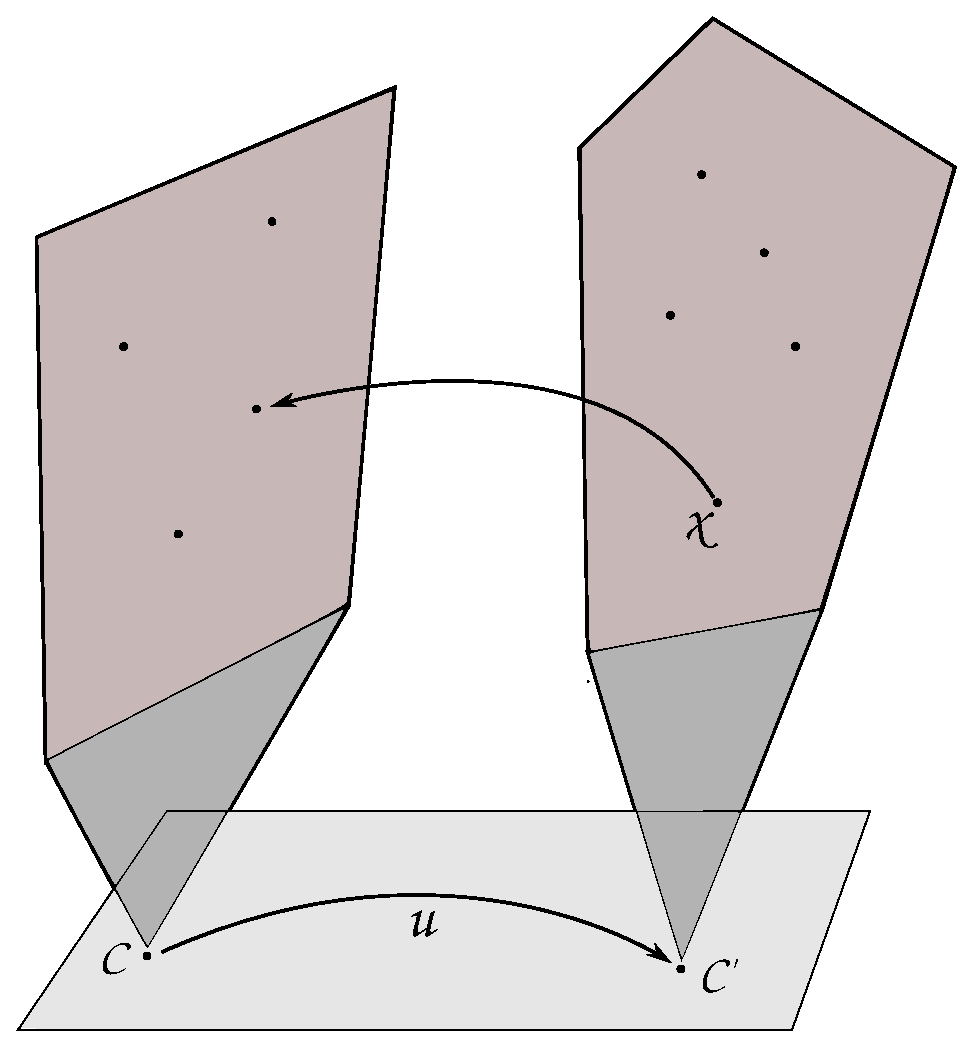
\includegraphics[width=.325\textwidth]{disegno.eps}
	\begin{tikzpicture}[>=stealth]
		\fill[gray!20,rounded corners] (0,0) rectangle (2,1);
		\node[font=\scriptsize] (C) at  (.25,.25) {$C$};
		\node[font=\scriptsize] (C') at (1.5,.5)  {$C'$};
		\draw[->] (C) -- (C') node[above, pos=.5] {$u$};
		%
		\draw[line width=4pt, gray!50, cap=round] (C) -- +(0,2);
		\draw[line width=4pt, gray!50, cap=round] (C') -- +(0,2.5);
		%
		\fill (1.5,2) circle (1pt) node (X') {};
		\fill (.25,1.5) circle (1pt) node (X) {};
		\draw[dashed,->] (X') -- (X);
		\node[above, font=\scriptsize] at (X') {$X'$};
		\node[above, font=\scriptsize] at (X) {$X$};
	\end{tikzpicture}
\end{center}
There is of course a similar correspondence for \emph{covariant} functors; the situation is conveniently depicted by the table
\begin{center}
	\begin{tabular}{ccc}
		\textbf{name}       & \textbf{variance}   & \textbf{condition} \\ \toprule
		fibration           & $\clC\to\Set$       &
		$
			\vcenter{\tiny \xymatrix@R=5mm{
		X \ar[r] \ar@{.}[d] & X'\ar@{.}[d]                             \\ \midrule
		pX \ar[r]_f         & C'
			}}
		$
		\\ \midrule
		opfibration         & $\clC^\op \to \Set$ &
		$
			\vcenter{\tiny \xymatrix@R=5mm{
		X \ar[r] \ar@{.}[d] & X'\ar@{.}[d]                             \\ \midrule
		C \ar[r]_f          & pX'
			}}
		$
		\\ \bottomrule
	\end{tabular}
\end{center}
% \f{La notazione va uniformata a questa scelta}
\begin{corollary}\label{da_collage}
	Given a profunctor $\fkR : \clA \pto \clB$, regarded as a functor $R : \clA^\op\times \clB \to \Set$, we can consider the category of elements $\elts{\clA^\op\times\clB}{R}$; this is often called the \emph{collage} or the \emph{graph} of $R$. In this case, we denote the category $\elts{\clA^\op\times\clB}{R}$ as $\clA\uplus_R\clB$, to stress the intuition that $R$ prescribes a way to glue together two categories $\clA,\clB$ specifying a set of `fake' arrows $R(A,B)$ that consistently interact with the arrows in $\clA,\clB$ (compare with \autoref{hint_at_collage}, and with \autoref{11_ramsey} below).
\end{corollary}
\begin{remark}\label{collage_explaned}
	The above definition deserves to be expanded a little more: from \autoref{eltsf} we get that the category $\clA\uplus_R\clB$ results as the category whose objects are those of the disjoint union $\clA_o\sqcup\clB_o$, and where the hom-set $\clA\uplus_R\clB(X,Y)$ is equal to
	\begin{enumtag}{c}
		\item $\clA(A,A')$ if $(X,Y)=(A,A')$ is a pair of objects in $\clA$;
		\item $\clB(B,B')$ if $(X,Y)=(B,B')$ is a pair of objects in $\clB$;
		\item $R(A,B)$ if $X=A$ is an object of $\clA$, and $Y=B$ is an object of $\clB$;
		\item empty in every other case.
	\end{enumtag}
	From this definition, it is evident that every profunctor $\fkR : \clA \pto \clB$ gives rise via its fibration of elements to a span
	\[ \vcenter{\xymatrix{
				& \clA\uplus_\fkR \clB \ar[dr]\ar[dl]& \\
				\clA  && \clB
			}} \]
\end{remark}
Thus, we have obtained a concrete model for a category that realises the generalised relation between $\clA,\clB$; the structure $\clA\uplus_R\clB$ is `carved' from $\clA,\clB$ separately, starting from (semi-)free relations witnessing the fact that $\fkR$ connects $\clA,\clB$ in a weak way. For example, if $\fkR : \clA^\op\times \clB \to \Set$ is the empty functor, then $\clA\uplus_R\clB$ is just he disjoint union of $\clA,\clB$; and if $\fkR$ is the functor constant at the singleton set, then $\clA\uplus_R\clB$ is the \emph{join} of $\clA,\clB$, i.e. the category $\clA\coprod\clB$ where exactly a single new morphism is added between each and every object of $\clA$ and of $\clB$ (but not in the opposite direction).
\begin{proposition}
	The collage construction of \autoref{da_collage} enjoys the following universal property: the category $\clA\uplus_R\clB$ fits into a cospan
	\[ \xymatrix{\clA \ar[r]^-J & \clA\uplus_R\clB & \ar[l]_-K \clB} \]
	where both functors $J,K$ are the obvious embeddings, and there exists a canonical natural transformation $\gamma : K_* \diamond \fkR \To J_*$ which is initial among all these: this means that given any other arrangement of profunctors 
	\[ \vcenter{\xymatrix{
		\clA \ar|-*=0@{|}@/^1pc/[drr]^(.6)\fkP\ar|-*=0@{|}[dr]^{J_*}\ar|-*=0@{|}[dd]_\fkR && \\ 
		& \clA\uplus_R\clB \ltwocell<\omit>{\gamma} \ar|-*=0@{|}@{.>}[r]^-{\fkU}& \clC \\ 
		\clB \ar|-*=0@{|}[ur]_{K_*}\ar|-*=0@{|}@/_1pc/[urr]_(.6)\fkQ & 
	}} \] like in this diagram of solid arrows, there exists a unique profunctor $\fkU : \clA\uplus_R\clB \pto \clC$ such that $\fkU\diamond J_*=\fkP$, $\fkU\diamond K_* = \fkQ$, and $\fkU * \gamma = \alpha$.
\end{proposition}
\section{Profunctors / Grothendieck construction}
\label{sec:org7dd09e1}
There are two possible ways to define a relation $R$ between two sets $A,B$:
\begin{enumtag}{r}
	\item \label{r_1} a relation $R$ is a subset of the cartesian product $A\times B$;
	\item \label{r_2} a relation $R$ is a function $A\times B \to \{0,1\}$.
\end{enumtag}
Note that the notion of `relation between $A$ and $B$' is inherently symmetric, in the sense that such $R$ can be regarded both as a relation `from' $A$ `to' $B$, and as a relation `from' $B$ `to' $A$.

Furthermore, every relation $R$ between sets $A,B$ gives rise to a \emph{Galois connection}
\[{}^R(\firstblank) :PA^\op \leftrightarrows PB : (\firstblank)^R \label{adjunzia} \]
between the powersets $PA=2^A$ and $PB = 2^B$: the set $U\subset A$ goes to the set ${}^RU$ of all $b$ such that $(a,b)\in R$ for all $a\in U$; in an exactly symmetric way, a set $V\subseteq B$ goes to the set
\[V^R = \{a\in A\mid (a,b) \in R,\, \forall b\in V\}.\]
Unwinding the definition, it is asy to verify that $V\subseteq{}^RU$ if and only if $U\subseteq V^R$, if and only if $U\times V\subseteq R$.
%\todo[inline]{La varianza di sta roba va controllata}

From here, using a process known as `categorification' \cite{baez_catego}, we can replace a two-valued relation $R : A\times B \to \{0,1\}$ with a \emph{set-valued} functor $\clA^\op\times\clB \to \Set$ between two (small) categories $\clA,\clB$.\footnote{The reason why the category $\clA$ is twisted with an `$^\op$' functor is that we want to bestow the hom functor $\hom_{\clA} : \clA^\op\times\clA \to \Set$ with the r\^ole of identity `profunctor'; in the categorification perspective, hom plays the r\^ole of the diagonal relation $R=\Delta : A\to A\times A$.} More precisely, we can give the following definition.
\begin{definition}[Profunctor]\label{def_profu}
	Let $\clA,\clB$ be two categories; a \emph{profunctor} $\fkR : \clA \pto \clB$ is a functor $\clA^\op\times\clB \to \Set$; we define the \emph{bicategory of profunctors} $\Prof$ having
	\begin{enumtag}{p}
		\item objects the small categories $\clA,\clB,\clC,\dots$;
		\item 1-cells the profunctors $\fkR : \clA \pto \clB$, and composition law between $\clA \overset{\fkR}{\pto} \clB \overset{\fkP}{\pto} \clC$ given by the assignment
		\[ (A,C)\mapsto \int^B \fkR(A,B)\times\fkP(B,C) \]
		(see \cite{} for the definition). The identity 1-cell is the hom functor $\hom_\clA : \clA^\op\times\clA \to \Set$;
		\item 2-cells $\fkR\To\fkR'$ the natural transfomations $\alpha : \xymatrix{\clA^\op\times\clB \rtwocell^{\fkR}_{\fkR'}{\alpha}& \Set}$.
	\end{enumtag}
\end{definition}
The intuition behind \autoref{def_profu} is that $\fkR(A,B)$ is the \emph{type} whose terms are all proofs that $(A,B)\in\clA^\op\times\clB$ are in a  `generalised relation' $\fkR$. This intuition agrees with the fact that when instead of $\Set$ a profunctor $\fkR$ takes values in the 0-dimensional category $\{0\le 1\}$, then the type of proofs that $R(A,B)$ is a yes/no space.

From here, one can build a rich and expressive theory; for our purposes, we are contempt with a careful analysis of the analogue of \ref{r_2} and \eqref{adjunzia} above: the latter is the scope of \autoref{sec:org1a423df}, we now concentrate on describing an ubiquitary technical tool in category theory.
\subsection{Grothendieck construction}
The Grothendieck construction is the tool allowing to formalise the equivalence between a relation understood as a function $R : A\times B \to \{0,1\}$, and a subset $R\subseteq A\times B$, when `relation' is understood in the sense of \autoref{def_profu} above, i.e. a profunctor $\fkR : \clA \pto \clB$.

Each such $\fkR$ can be realised as a suitable `fibration' $p_\fkR : \clE \to \clA^\op\times\clB$, that in turn uniquely determines $\fkR$.
We now recall a few basic definitions.
\begin{definition}\label{eltsf}
	Let $\clC$ be an ordinary category, and let $W : \clC\to \Set$ be a functor; the \emph{category of elements} $\elts{\clC}{W}$ of $W$ is the category which results from the pullback
	\[
		\xymatrix{
			\elts{\clC}{W}\ar[r]\ar[d] \pb & \Set_* \ar[d]^U \\
			\clC \ar[r]_W & \Set
		}
	\]
	where $U : \Set_*\to\Set$ is the forgetful functor which sends a pointed set to its underlying set.

	More explicitly, $\elts{\clC}{W}$ has objects the pairs $(C\in\clC, u\in WC)$, and morphisms $(C,u)\to (C',v)$ those $f\in \clC(C,C')$ such that $W(f)(u)=v$.
\end{definition}
\begin{definition}[Discrete fibration]
	\label{def:dfib}
	A \emph{discrete fibration} of categories is a functor $G : \clE \to \clC$ with the property that for every object $E\in\clE$ and every arrow $p : C\to GE$ in $\clC$ there is a unique $q : E'\to E$ `over $p$', i.e. such that $Gq=p$.
\end{definition}
Taking as morphisms between discrete fibrations the morphisms in $\Qat/\clC$, we can define the category $\DFib(\clC)$ of discrete fibrations \emph{over} $\clC$.
\begin{proposition}\label{fibelem}
	The category of elements $\elts{\clC}{W}$ of a functor $W : \clC\to \Set$ comes equipped with a canonical \emph{discrete fibration} to the domain of $W$, which we denote $\Sigma : \elts{\clC}{W}\to \clC$, defined forgetting the distinguished element $u\in Wc$.
\end{proposition}
With this terminology at hand, we can consider the \emph{category of elements} \ref{eltsf} of a functor $F : \clC\to \Set$; this sets up a functor from $\Qat(\clC,\Set)$ to the category of discrete fibrations over $\clC$: the Grothendieck construction asserts that this is an equivalence of categories.%, as defined in \ref{def:equcat}.
\begin{theorem}\label{thm:equconfib}
	There is an equivalence of categories
	\[
		\Qat(\clC^\op,\Set) \to \DFib(\clC)
	\]
	defined by the correspondence sending $F\in\Qat(\clC,\Set)$ to its \emph{fibration of elements}  $\Sigma_F : \elts{\clC}{F} \to \clC$.
\end{theorem}
The inverse correspondence sends a discrete fibration $\Phi : \clE \to \clC$ to the functor whose action on objects and morphisms is depicted in the following image: an object $C\in\clC$ goes to the fiber $\Phi^{-1}C$ in $\clE$, that since $\Phi$ is a discrete fibration is a discrete subcategory of $\clE$, hence a set; a morphism $u : C\to C'$ defines a function $\Phi^{-1}C' \to \Phi^{-1}C$: the object $X'\in\Phi^{-1}C'$ goes to the (unique) object $X$ in the fiber over $C$, that is the domain of the arrow $v$ such that $\Phi v=u$.
\begin{center}
	% 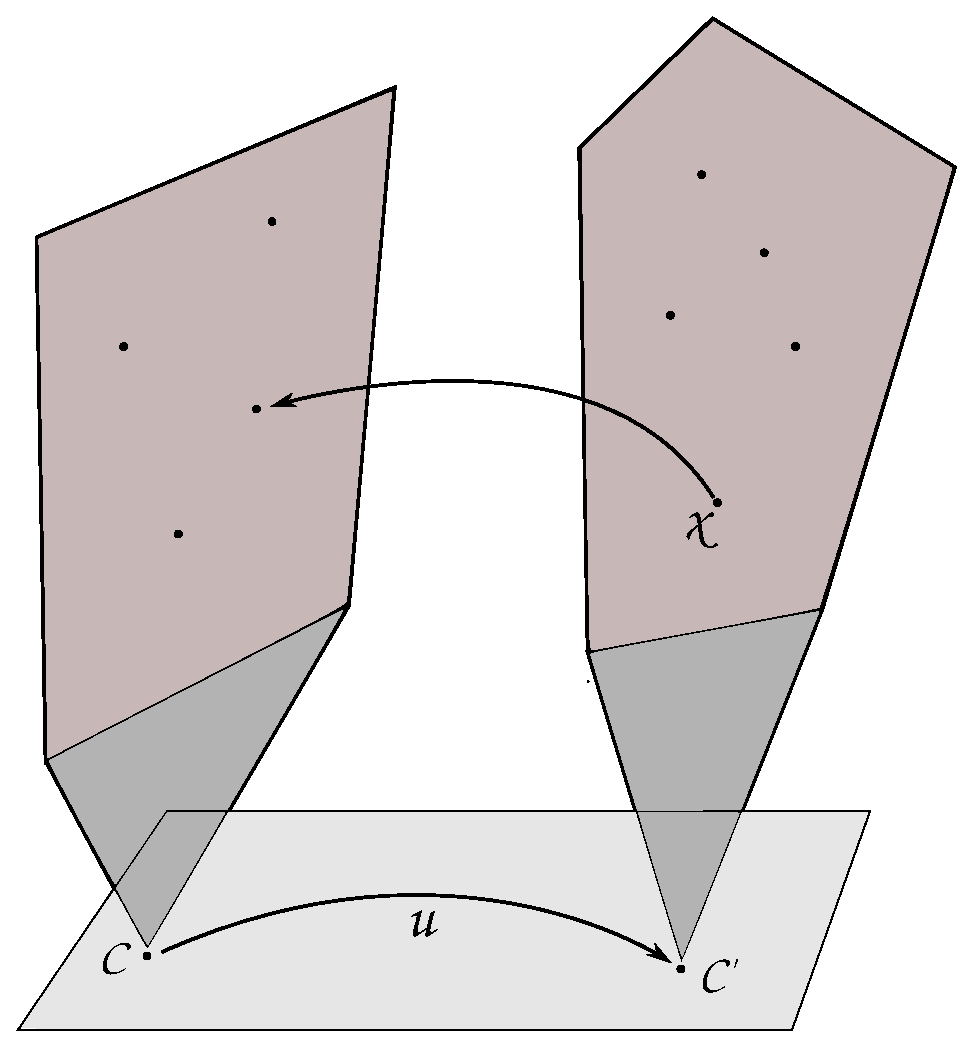
\includegraphics[width=.325\textwidth]{disegno.eps}
	\begin{tikzpicture}[>=stealth]
		\fill[gray!20,rounded corners] (0,0) rectangle (2,1);
		\node[font=\scriptsize] (C) at  (.25,.25) {$C$};
		\node[font=\scriptsize] (C') at (1.5,.5)  {$C'$};
		\draw[->] (C) -- (C') node[above, pos=.5] {$u$};
		%
		\draw[line width=4pt, gray!50, cap=round] (C) -- +(0,2);
		\draw[line width=4pt, gray!50, cap=round] (C') -- +(0,2.5);
		%
		\fill (1.5,2) circle (1pt) node (X') {};
		\fill (.25,1.5) circle (1pt) node (X) {};
		\draw[dashed,->] (X') -- (X);
		\node[above, font=\scriptsize] at (X') {$X'$};
		\node[above, font=\scriptsize] at (X) {$X$};
	\end{tikzpicture}
\end{center}
There is of course a similar correspondence for \emph{covariant} functors; the situation is conveniently depicted by the table
\begin{center}
	\begin{tabular}{ccc}
		\textbf{name}       & \textbf{variance}   & \textbf{condition} \\ \toprule
		fibration           & $\clC\to\Set$       &
		$
			\vcenter{\tiny \xymatrix@R=5mm{
		X \ar[r] \ar@{.}[d] & X'\ar@{.}[d]                             \\ \midrule
		pX \ar[r]_f         & C'
			}}
		$
		\\ \midrule
		opfibration         & $\clC^\op \to \Set$ &
		$
			\vcenter{\tiny \xymatrix@R=5mm{
		X \ar[r] \ar@{.}[d] & X'\ar@{.}[d]                             \\ \midrule
		C \ar[r]_f          & pX'
			}}
		$
		\\ \bottomrule
	\end{tabular}
\end{center}
\todo[inline]{La notazione va uniformata a questa scelta}
\begin{corollary}
	Given a profunctor $\fkR : \clA \pto \clB$, regarded as a functor $R : \clA^\op\times \clB \to \Set$, we can consider the category of elements $\elts{\clA^\op\times\clB}{R}$; this is often called the \emph{collage} or the \emph{graph} of $R$. In this case, we denote the category $\elts{\clA^\op\times\clB}{R}$ as $\clA\uplus_R\clB$, to stress the intuition that $R$ prescribes a way to glue together two categories $\clA,\clB$ specifying a set of `fake' arrows $R(A,B)$ that consistently interact with the arrows in $\clA,\clB$ (compare with \autoref{hint_at_collage}, and with \autoref{11_ramsey} below).
\end{corollary}
\begin{remark}
	The above definition deserves to be expanded a little more: from \autoref{} we get that the category $\clA\uplus_R\clB$ results as the category whose objects are those of the disjoint union $\clA_o\sqcup\clB_o$, and where the hom-set $\clA\uplus_R\clB(X,Y)$ is equal to
	\begin{enumtag}{c}
		\item $\clA(A,A')$ if $(X,Y)=(A,A')$ is a pair of objects in $\clA$;
		\item $\clB(B,B')$ if $(X,Y)=(B,B')$ is a pair of objects in $\clB$;
		\item $R(A,B)$ if $X=A$ is an object of $\clA$, and $Y=B$ is an object of $\clB$;
		\item empty in every other case.
	\end{enumtag}
\end{remark}
Thus, we have obtained a concrete model for a category that realises the generalised relation between $\clA,\clB$; the structure $\clA\uplus_R\clB$ is `carved' from $\clA,\clB$ separately, starting from (semi-)free relations witnessing the fact that $\fkR$ connects $\clA,\clB$ in a weak way. For example, if $\fkR : \clA^\op\times \clB \to \Set$ is the empty functor, then $\clA\uplus_R\clB$ is just he disjoint union of $\clA,\clB$; and if $\fkR$ is the functor constant at the singleton set, then $\clA\uplus_R\clB$ is the \emph{join} of $\clA,\clB$, i.e. the category $\clA\coprod\clB$ where exactly a single new morphism is added between each and every object of $\clA$ and of $\clB$ (but not in the opposite direction).
\section{Theories and models}\label{sec_4_theories}
\label{sec:orge02f333}
In this section we exploit the terminology established before.
\begin{definition}[Theory]\label{teoria}
	A \emph{theory} $\clL$ is the syntactic category $\clT_L$ (cf. \cite[II.11]{lambek1988introduction}) of a type theory $L$.
\end{definition}
The reader interested in how the construction of $\clT_L$ goes can take from \cite{lambek1988introduction} as standard reference, or \cite{abramskyno} for a shorter survey, in the simple case $L$ admits product and function types.
\begin{definition}[World, Yuggoth]\label{mondo_yalda}
	A \emph{world} is a large category $\clW$; a \emph{Yuggoth}\footnote{\emph{Yuggoth} (also \emph{Iukkoth}, or {\yugg} in Chtuvian language) is an enormous trans-Neptunian planet whose orbit is perpendicular to the ecliptic plane of the solar system. A Yuggoth is a world so big to inspire a sense of unfathomable awe.} is a world that, as a category, admits all small colimits.
\end{definition}
\begin{definition}[Canvas, science]\label{canvas_scienza}
	Given a theory $\clL$ and a world $\clW$, a $\clL$-\emph{canvas} of $\clW$ is a functor
	\[\xymatrix{\clL \ar[r]^\phi & \clW.}\]

	A canvas $\phi : \clL \to \clW$ is a \emph{\science} if $\phi$ is a dense functor.
\end{definition}
\begin{remark}\label{remark_yuggoth_1}
	The NR paradigm exposed in \autoref{nr_para} now entails that given a canvas $\phi : \clL \to \clW$
	\begin{itemize}
		\item If $\clW$ is a world, we obtain a \emph{representation} functor
		      \[ \xymatrix{\clW \ar[r] & [\clL^\op, \Set];} \label{mvndvs}\]
		      this means: given a canvas $\phi$ of the world, the latter leaves an image on the canvas.
		\item If in addition $\clW$ is a Yuggoth, we obtain a NR-adjunction
		      \[\xymatrix{\clW \ar@<3pt>[r] & \ar@<3pt>[l] [\clL^\op, \Set];}\]
		      this has to be interpreted as: if $\clW$ is sufficiently expressive, then models of the theory that explains $\clW$ through $\phi$ can be used to acquire a two-way knowledge. Phenomena have a theoretical counterpart in $[\clL^\op,\Set]$ via the nerve; theoretical objects strive to describe phenomena via their realisation.
		\item If an $\clL$-canvas $\phi : \clL \to \clW$ is a \science, `the world' is a full subcategory of the class of all modes in which `language' can create interpretation.
	\end{itemize}
\end{remark}
\begin{remark}\label{remark_yuggoth_2}
	The terminology is chosen to inspire the following idea in the reader: science strives to define \emph{theories} that allow for the creation of world representations; said representations are descriptive when there is dialectic opposition between world and models; when such representation is faithful, we have reduced `the world' to a piece of the models created to represent it.

	The tongue-in-cheek here is: a science in the usual sense of the world can never attain the status of a \science, if not potentially; this because all of its attempts at describing the world are partial. But if the chosen language is powerful enough, even a small fragment of it can result in a `free linguistic category' (precisely $[\clL^\op,\Set]$) that is large enough to encompass $\clW$ completely.
	
	In this perspective, attempts to generate scientific knowledge are the attempts of
	\begin{itemize}
		\item recognizing the world $\clW$ as a sufficiently expressive object for it to contain phenomena and information;
		\item carve a language $L$, if necessary from a small subset of $\clC$, that is sufficiently `compact', but also sufficiently expressive for its syntactic category to admit a representation into the world;
		\item obtaining an \emph{adjunction} between $\clW$ and models of the worlds obtained as models of the syntactic theory $\clL$; this is meant to generate models starting from observed phenomena, and to predict new phenomena starting from models;
		\item obtaining that `language is a dense subset of the world', by this meaning that the adjunction outlined above is sufficiently well-behaved to describe the world as a fragment of the semantic interpretations obtained from~$\clL$.
	\end{itemize}
	It is evident that there is a tension between two opposite feature that $\clL$ must exhibit; it has to be not too large to remain tractable, but on the other hand it must be large enough in order to be able to speak about `everything' it aims to describe.
\end{remark}
Regarding our definition of \science, we can't help but admit we had the following definition in mind \cite[2.1]{biologia}, regarded with a pair of category theorist' goggles:
\begin{definition*}[\protect{\cite[2.1]{biologia}}]
	A \emph{scientific theory} $\clT$ consists of a formal structure $F$ and a class of interpretations $M_i$, shortly denoted as $\clT=\langle F,M_i\mid i\in I\rangle$. The structure $F$ consists on its won right of
	\begin{itemize}
		\item a language $\clL$, in which it is possible to formulate propositions. If $\clL$ is fully formalised, it will consist of a finite set of symbols, and a finite set of rules to determine which expressions are well-formed. This is commonly called \emph{technical language};
		\item A set $A$ of `axioms' or `postulates' in $\clL^\star$;
		\item A \emph{logical apparatus} $R$, whose elements are rules of inference and logical axioms, allowing to prove propositions.
	\end{itemize}
\end{definition*}
The language of category theory allows for a refined rephrasing of the previous definition: we say that a \emph{$\clS$-scientific theory} is the following arrangement of data:
\begin{enumtag}{st}
	\item a formal language $\clL$;
	\item the syntactic category $T_\clL$, obtained as in \cite[II.11]{lambek1988introduction};
	\item the category of functors $[T_\clC, \clS]$, whose codomain is a Yuggoth.
\end{enumtag}
More than often, our theories will be $\Set$-scientific: in such case we just omit the specification of the semantic Yuggoth, and call them \emph{scientific theories}.

Since the category $[T_\clC, \Set]$ determines $\clL$ and $T_\clL$ completely, up to Cauchy-completion \cite{borceuso-cauchy}, we can see that the triple $(\clL, T_\clL, [T_\clL,\Set])$ can uniquely be recovered from its model category $[T_\clC, \Set]$. We thus comply to the additional abuse of notation to call `scientific theory' the category $[T_\clL,\Set]$ for some $T_\clL$.

So, a `coherent correspondence linking expressions of $\clF$ with semantic expressions' boils down to a functor; this is compatible with \cite[2.1]{biologia}, and in fact an improvement (the mass of results in category theory become readily available to speak about --scientific-- theories; not to mention that the concept of `formal structure' is never rigorously defined throughout \cite{biologia}).

%\subsection{The first rough attempt of some infant god}
Let us consider two categories $\clO,\clT$, respectively the \emph{observational} and the \emph{theoretical}. Even though their origin is never examined further, it is fruitful to think that $\clO,\clT\subseteq \clW$, i.e. that they are `carved' from the world, building respectively on the tangible experience (for $\clO$) and on a linguistic structure (for $\clL$).

If $\clW$ is a Yuggoth each pair of canvases
\[ \xymatrix{
		\clO \ar[r]^-\psi & \clW & \ar[l]_-\phi \clT
	} \label{2_canvases}\] gives rise, according to \eqref{mvndvs}, to representations
\[ \xymatrix{
	[\clO^\op,\Set] \ar@<.5em>[r] & \ar@<.5em>[l]^-{N_\psi} \clW \ar@<-.5em>[r]_-{N_\phi} \ar@{}[r]|-\perp \ar@{}[l]|-\perp & \ar@<-.5em>[l] [\clT^\op,\Set]
	} \label{2_reps}\]
The leftmost category is the category we have experimental access, starting from the fragment $\clO \subseteq \clW$ we can observe. The rightmost category is the category of symbols we can speak of, trying to reproduce the observed behaviour.
\begin{definition}
	We refine the terminology introduced above to speak of a \emph{theoretical} (resp., a \emph{observational}) \emph{science}, assuming that $\phi$ (resp., $\psi$) is a \science.
\end{definition}
Assuming that $\phi : \clT \to \clW$ is a theoretical \science, now, the representation functor $\clW \to [\clT^\op,\Set]$ above acquires a left adjoint.
\section{The tension between observational and theoretical}
\label{sec:orge11c3c4}
When working with categorified relations, it is unnatural and somewhat restrictive to take into account a two-element set for the possible values a proposition(al function) `$(a,b)\in R$' can assume; instead we would like to consider an entire \emph{space} of such values, or rather a type of proofs that $(a,b)\in R$ is true. Again, this idea is best appreciated when thinking that the same proposition 
\begin{center}
	\begin{minted}{haskell}
	(n : Nat) -> (m : Nat) ->  n + m = m + n 
	\end{minted}
\end{center}
when encoded in any (sufficiently strongly-typed) DSL, can be interpreted as either the \emph{proposition} `given $n$ and $m$ natural numbers, their sum is a commutative operation' or as the \emph{type} \mil{n + m} $\equiv$ \mil{m + n} whose elements are the proofs that $n+m$ is in fact equal to $m+n$.

This intuition is based on the well-known proportion
\begin{center}
	truth values : proposition = section : presheaf
\end{center}
inspired by the `proposition as types' paradigm. In simple terms, categorifying a proposition $P : X\to \{0,1\}$ that can or cannot hold for an element $x$ of a set $X$, we shall marry the constructive church and say that there is an entire \emph{type} $PC$, image of an object $C\in\clC$ under a functor $P : \clC \to \Set$, whose \emph{terms} are the \emph{proofs} that $PC$ holds true. This is nothing but the propositions-as-types philosophy, in (not so much) disguise: \cite{hottbook,wadler,martin1984intuitionistic}

The important point for us is that the dialectical tension between observational and theoretical can be faithfully represented through profunctor theory; one can think of propositional functions as relations $(x,y)\in R$ iff the pair $x,y$ renders $\phi$ true; we use this idea, suitably adapted to our purpose and categorified. This very natural extension of propositional calculus, pushed to its limit, yields the following reformulation of the `tension between observational and theoretical' of \cite{u,v,w}
\begin{definition}\label{11_ramsey}
	Let $\clT,\clO$ be two small categories, dubbed respectively the \emph{theoretical} and the \emph{observational} settings. A \emph{$(1,1)$-ary Ramsey map} is merely a profunctor
	\[\fkK : \clT^\op \pto \clO\]
	or, spelled out completely, a functor $\fkK : \clT\times \clO \to \Set$.
\end{definition}
By accepting the prefix ``$(1,1)$-'' we ask the reader the leap of faith that \autoref{11_ramsey} is but a particular instance of a more general definition, \autoref{mn_ramsey}. 

Before delving into this generalisation in \autoref{multiramsey}, however, a more elementary remark is in order: there is a particularly elementary recipe to generate $(1,1)$-ary Ramsey maps.
\begin{example}
	Every functor $F : \clA \to \clB$ gives rise to a profunctor $F_* := \clB(1,F) : \clB^\op\times \clA\to\Set$ and a profunctor $F^* := \clB(F,1) : \clA^\op\times\clB \to \Set$ as in \autoref{nervereal}; the two functors are mutually adjoint, $F^*\dashv F_*$, see \cite[6.2]{Bor2}. This yield an example of what we call \emph{representable} Ramsey maps.
\end{example}
\begin{definition}[Observational and theoretical nucleus]\label{nuclei}
	Let $\fkR : \clT^\op\times \clO \to\Set$ be a Ramsey map, and $\hat R : \clO \to [\clT^\op,\Set]$ the associated canvas. Let
	\[ \Lan_{\yon_\clO}\hat R : [\clO^\op,\Set] \leftrightarrows [\clT^\op,\Set] : N_{\hat R} \]
	be the adjunction between presheaf categories determined by virtue of \autoref{equ_prof_cocont}. Let us consider the equivalence of categories between the fixpoints of the monad $T = N_{\hat R}\circ\Lan_{\yon_\clO}\hat R$ and the comonad $S=\Lan_{\yon_\clO}\hat R\circ N_{\hat R}$.
	
	This is the equivalence between the \emph{observational nucleus} $Fix(T)\subseteq [\clO^\op,\Set]$ and the \emph{theoretical nucleus} $Fix(S)\subseteq [\clT^\op,\Set]$.
\end{definition}
\begin{remark}
	Observational nucleus and theoretical nucleus always form equivalent categories; the tension in creating a satisfying image of reality as it is observed oscillates between the desire to enlarge as much as possible the subcategory of $[\clO^\op,\Set]$ with which our theoretical model is equivalent, where we can have access to $\clT, [\clT^\op, \Set]$ only.
\end{remark}
The chain of observations in \autoref{inducing_herme} motivates the following definition.
\begin{definition}
	In a display of categories like \eqref{2_canvases} we say that 
	\begin{itemize}
		\item A \emph{fundamental cell} is a natural transformation $\psi^* \To R(\phi,1)$;
		\item In $\clW$ \emph{hermeneutics is possible} if the right Kan extension $\bk{\phi,\psi} := \Ran_{\phi^*}\psi^*$ exists \emph{as a functor} (note that it always exists as a profunctor).
	\end{itemize}
	If hermeneutics is possible in $\clW$, and $R : \clO \pto \clT$ is a Ramsey map, any fundamental cell induces a natural transformation 
	\[ \varpi : N_{\hat R} \To \bk{\phi,\psi} \]
\end{definition}
\begin{remark}
	The reader might have observed, now, that there is nothing in their mere syntactical presentation allowing to tell apart the observational and the theoretical category; this can be justified with the fact that the bicategory $\Prof$ of \autoref{def_profu} is endowed with a canonical self-involution, exchanging the r\^ole of domain and codomain of 1-cells, and thus of the theoretical and observational category $\clT,\clO$.
	
	This is perhaps of some help in solving the conundrum posed by the existence of `fictional objects'. Sherlock Holmes clearly is the object of a theoretical category. Gandhi is the object of an observational category. But as linguistic objects they can't be told apart completely; they can be at most separated by a profunctor embedding the former in a realistic but fictitious model (that is, for example, the Reichenbach falls), and representing the latter as part of a fictional model (for example, as part of a movie directed by R. Attenborough).
\end{remark}
\begin{remark}\label{multiramsey}
	The notion of Ramsey map as given above is unnecessarily restrictive, and does not account for many sorts of configurations that can occur in practice:
	\begin{itemize}
		\item a single observational token $O$ can't be described by a single theoretical token $T_1$, but instead needs $T_1,\dots,T_r$;
		\item inverting the r\^oles, a single theoretical token describes not only $O$, but different $O_1,\dots,O_s$.
	\end{itemize}
	Thus we must admit \emph{multiple} arguments for the domain and codomain of a Ramsey map. This yields the notion of a \emph{$(n,m)$-ary Ramsey map}.
\end{remark}
\begin{remark}\label{resoudre_la_tension}
	The clearest possible sense in which the profunctorial approach `resolves' the tension between observational and theoretical is that the Gro\-then\-dieck construction associated to a profunctor $\fkR : \clT \pto \clO$ yields a category where the two `worlds', one carved from perception, and the other concocted from language, live harmoniously together. All in all, said tension is just an incarnation of the tension between speakable and unspeakable: given a Ramsey map $\fkR : \clT \pto \clO$, the equivalence between its theoretical and observational nuclei is an equivalence between the speakable (subclass of $[\clT^\op,\Set]$), with the observable (subclass of $[\clO^\op,\Set]$); what lies outside this equivalence in the latter category is observable but `unspeakable' in the strongest possible sense.
\end{remark}

% \section{Ramseyfication and beyond: generalised profunctors}
\label{sec:org50db6c2}
We can generalise the definition above to encompass Ramsey sentences:
\begin{definition}\label{mn_ramsey}
	Let $\clT,\clO$ be two categories; a \emph{Ramsey map}, or a \emph{$(n,m)$-ary Ramsey map} is a profunctor $\fkK : \clT^n \pto \clO^m$; note that we allow $n,m$ to be zero; in that case, $\clA^0$ is understood to be the terminal category $\boldsymbol{1}$.
\end{definition}
The intuition behind this definition is as follows: given $\uT\in\clT^n, \uO\in\clO^m$, the set $\fkK(\uT, \uO)$ represents the type of proofs that the observational tuple $\uO$ admits a description in terms of the theoretical tuple $\uT$.

This formalism allows to speak about particular worlds, obtained as presheaf categories over observational $\clO$; if $\clT, \clO$ is a theoretical pair, we can instantiate \autoref{nervereal} above in the particular case where $\clW = [\clO^\op, \Set]$ (observe that in this case $\clW$ is a Yaldabaoth). We can thus address a certain number of questions, arising from the canonical adjunction obtained by virtue of \autoref{equ_prof_cocont}:% and \autoref{}:
\[
	\xymatrix{ [(\clO^m)^\op, \Set] \ar@<3pt>[r] & \ar@<3pt>[l] [(\clT^n)^\op, \Set];}
\]
It is worth to mention that since the diagram
\[
	\vcenter{\xymatrix{
			(\clO^m)^\op \ar[rr]\ar[dr]&& [(\clT^n)^\op, \Set] \ar[dl]\\
			& [(\clO^m)^\op, \Set]
		}}
\]
is pseudocommutative, the composition $L\circ y$ s equal to (the mate of) $\fkK$. This means: $\clO$-models, when interpreted inside $\clT$-models, carry representations corrisponding to the observational tokens interpreted in $\clT$-models; that is, the representation is coherent over observational tokens, that is\dots

\fo{Vanno messi a posto tutti i domini qua}
\begin{remark}[Ramseyfication and translation functors]\label{carnap_translation_functors}
	Assume that there exists an adjunction 
	\[ 
		L : \clT \leftrightarrows \clO : F
	\]
	between the theoretical and the observable. Following Carnap, we might assume that $F : \clO \hookrightarrow \clT$, and thus $G$ is a right translation functor for $(\clT, \clO)$.

	In these assumptions, given a Ramsey map $\fkK : \clO \pto\clT$ the function term
	\[\lambda \uO\lambda\uX . \fkK(\uO, \uX)\]
	can be pre-composed with $F$ obtaining
	\[\lambda \uO\lambda\uO'.\fkK(\uO, F\uO').\]
	We say that a translation adjunction $(L,F)$ is `$\fkK$-admissible' (denoted $L \dashv_\fkK F$) when there is a natural isomorphism $\fkK(L,1)\cong\fkK(1,F)$.
\end{remark}
The property of $\fkK$-admissibility for a pair of functors is in general difficult to assess; nevertheless, there are interesting properties for the relation $F\dashv_\fkK G$: for example
\begin{theorem}
	Let $F : \clA \leftrightarrows \clB: G$ be a pair of functors in opposite directions; let $\fkK : \clB \pto \clA$ be a profunctor; if $F\dashv_\fkK G$, then there is a `genuine' adjunction 
	\[ F^e : \clA\uplus_\fkK\clB \leftrightarrows \clA\uplus_\fkK\clB : G^e \]
	`extended' to the category of elements of $\fkK$.
\end{theorem}
\section{Ramseyfication and beyond: generalised profunctors}
\label{sec:org50db6c2}
We can generalise the definition above to encompass Ramsey sentences:
\begin{definition}\label{mn_ramsey}
	Let $\clT,\clO$ be two categories; a \emph{Ramsey map}, or a \emph{$(n,m)$-ary Ramsey map} is a profunctor $\fkK : \clT^n \pto \clO^m$; note that we allow $n,m$ to be zero; in that case, $\clA^0$ is understood to be the terminal category $\boldsymbol{1}$.
\end{definition}
The intuition behind this definition is as follows: given $\uT\in\clT^n, \uO\in\clO^m$, the set $\fkK(\uT, \uO)$ represents the type of proofs that the observational tuple $\uO$ admits a description in terms of the theoretical tuple $\uT$.

This formalism allows to speak about particular worlds, obtained as presheaf categories over observational $\clO$; if $\clT, \clO$ is a theoretical pair, we can instantiate \autoref{nervereal} above in the particular case where $\clW = [\clO^\op, \Set]$ (observe that in this case $\clW$ is a Yaldabaoth). We can thus address a certain number of questions, arising from the canonical adjunction obtained by virtue of \autoref{equ_prof_cocont}:% and \autoref{}:
\[
	\xymatrix{ [(\clO^m)^\op, \Set] \ar@<3pt>[r] & \ar@<3pt>[l] [(\clT^n)^\op, \Set];}
\]
It is worth to mention that since the diagram
\[
	\vcenter{\xymatrix{
			(\clO^m)^\op \ar[rr]\ar[dr]&& [(\clT^n)^\op, \Set] \ar[dl]\\
			& [(\clO^m)^\op, \Set]
		}}
\]
is pseudocommutative, the composition $L\circ y$ s equal to (the mate of) $\fkK$. This means: $\clO$-models, when interpreted inside $\clT$-models, carry representations corrisponding to the observational tokens interpreted in $\clT$-models; that is, the representation is coherent over observational tokens, that is\dots
\begin{remark}[Ramseyfication and translation functors]\label{carnap_translation_functors}
	Assume that there exists an adjunction 
	\[ 
		F : \clO \leftrightarrows \clT : G
	\]
	between the theoretical and the observable. Following Carnap, we might assume that $F : \clO \hookleftarrow \clT$, and thus $G$ is a right translation functor for $(\clT, \clO)$.

	In these assumptions, given a higher Ramsey map $\fkK : \clO \times \clT \to \Set$ the function term
	\[\lambda \uO\uX . \fkK(\uO, \uX)\]
	can be pre-composed with $G$ obtaining
	\[\lambda \uT.\fkK(F\uT, \uT)\]
	whenever there is an adjunction $F : \clO \leftrightarrows \clT : G$ between the theoretical and the observable. We say that a translation adjunction $(F,G)$ is `$\fkK$-admissible' when there is an isomorphism $\fkK(F\uT,\uT')\cong\fkK(\uT,G\uT')$.

	% This, together with the fact that $F\dashv G$ iff $F^*\cong G_*$ iff $G^*\cong F_*$, suggests a fruitful intuition: in presence of a `botched isomorphism' between observational and theoretical, witnessed by the adjunction $(F,G)$, we consider the theoretical trace left by the (image under $F$ of the) observational tokens, so that the dependency of $\fkK$ from $\uT$ is `eliminated' by means of the adjunction.

	% Clearly, the opposite procedure is possible: the adjunction $(F,G)$ allows to consider the observational trace left by the image of a theoretical token $\uT$ under $G$, so that
	% \[ \exists \uX . \fkK(\uO, \uX) \equiv \lambda \uO.\fkK(G\uT, \uT) \]
\end{remark}

\bibliography{../allofthem}{}
\bibliographystyle{siam}
\end{document}
